\chapter{Progettazione concettuale}
    \section{Class Diagram del dominio del problema}
        Dall'analisi dei requisiti costruiamo il Class Diagram del dominio del problema.\\
        In particolare, il modello concettuale basato sull'analisi dei requisiti permetterà di creare un modello efficace per la gestione del personale e delle attività svolte nell'azienda.\\
        Il modello dovrà tenere in considerazione le due tipologie di dipendenti con le relative caratteristiche e responsabilità, i laboratori, i progetti e le attrezzature.\\
        %Class Diagram costruito con StarUML
        \begin{figure}[htbp!]
            \centering
                \vspace{2\baselineskip}
                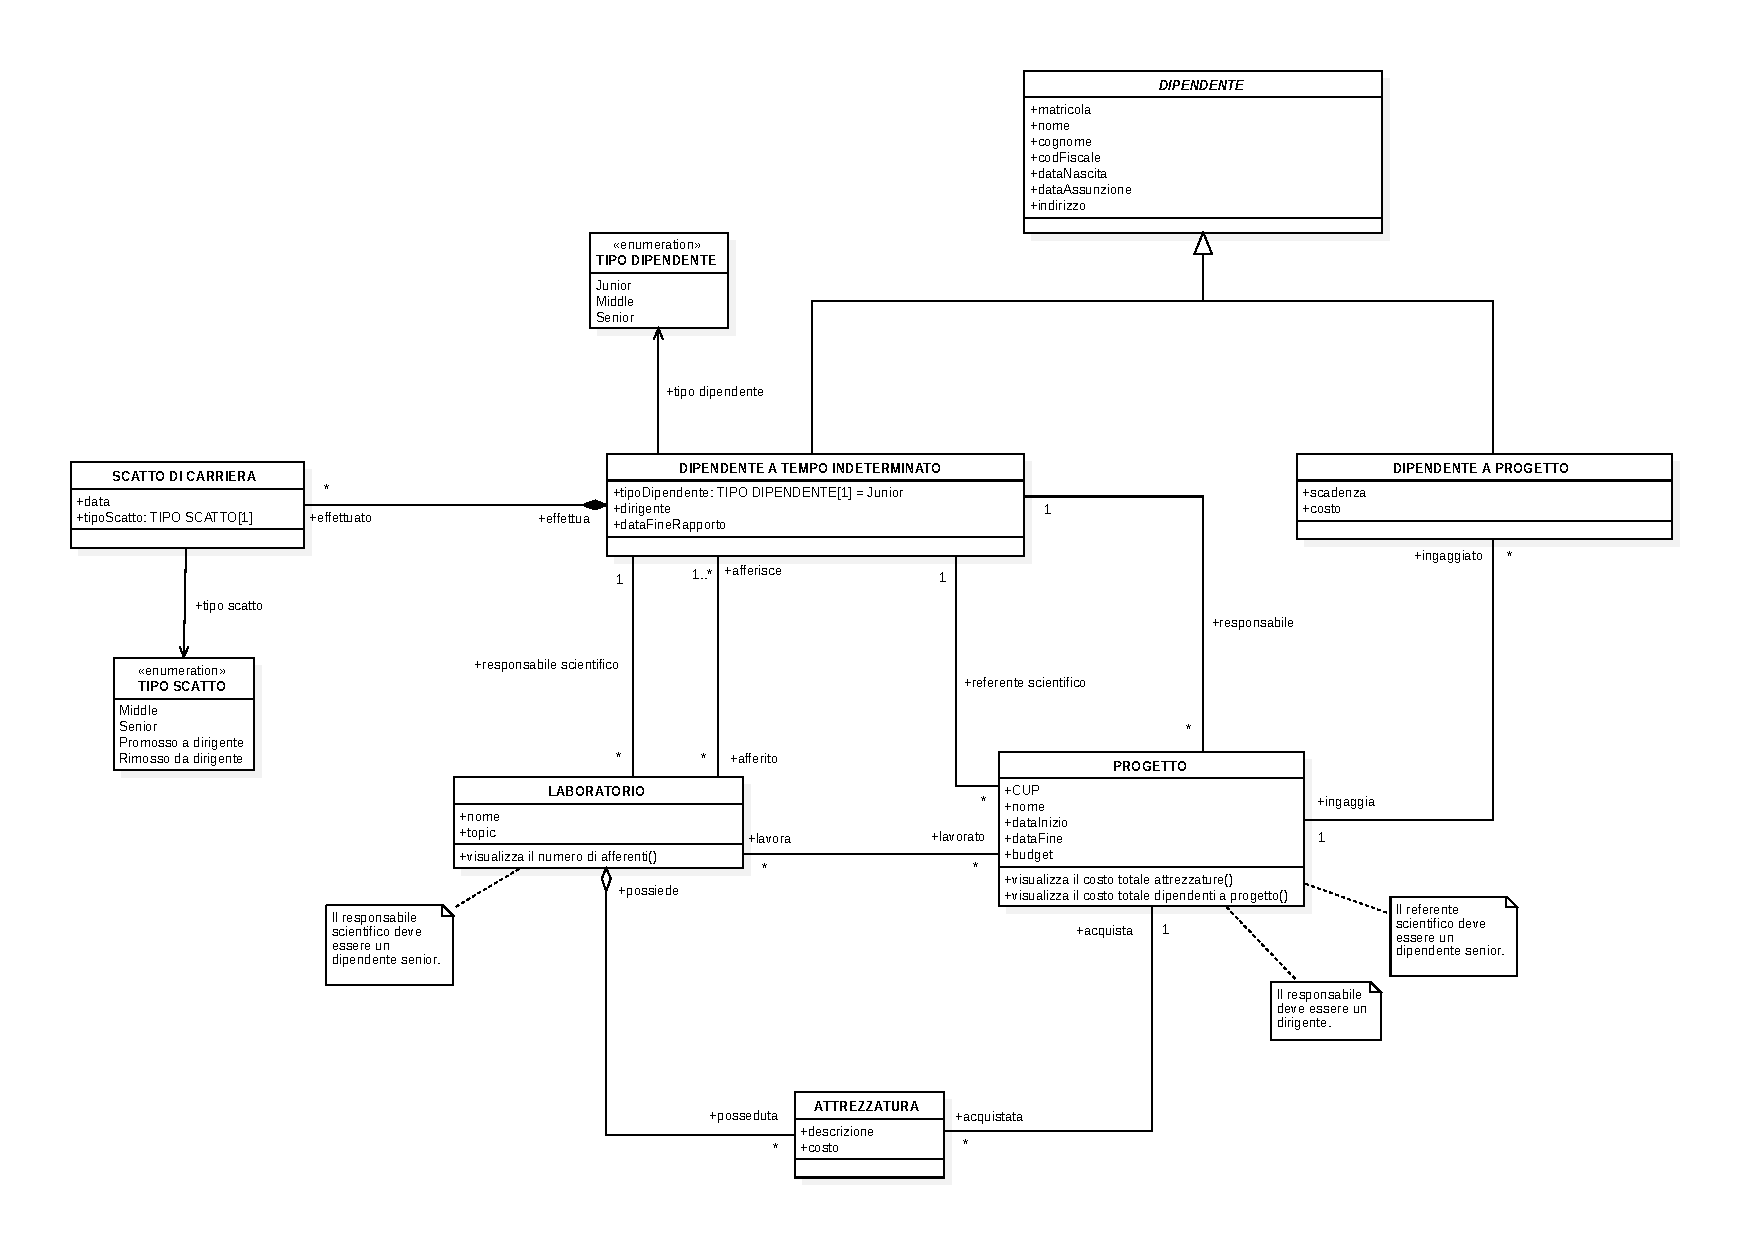
\includegraphics[width=\linewidth]{Immagini/Diagrammi/Class Diagram/Class diagram del dominio del problema.pdf}
            \caption{Class Diagram del dominio del problema}
            \label{fig:Class Diagram del dominio del problema}
        \end{figure}

    \section{Dizionario delle classi}
        \begin{tabular}{|C{3.5cm}|L{11.2cm}|}
            \hline
            \multicolumn{1}{|c|}{\textbf{Classe}} & \multicolumn{1}{c|}{\textbf{Descrizione}}\\  
            \hline
                DIPENDENTE &
                La classe "Dipendente" è una generalizzazione di "Dipendente a tempo indeterminato" e "Dipendente a progetto". Queste ultime due classi erediteranno gli attributi di "Dipendente": la matricola, il nome, il cognome, il codice fiscale, l'indirizzo di residenza, la data di nascita, la data di assunzione.\\
            \hline
                DIPENDENTE CON CONTRATTO A TEMPO INDETERMINATO &
                La classe "Dipendente a tempo indeterminato" rappresenta i dipendenti assunti con contratto a tempo indeterminato dall'azienda. Eredita da "Dipendente". Agli attributi di "Dipendente", aggiungiamo la data di fine rapporto (ovvero la data in cui eventualmente smette di prestare servizio nell'azienda), un attributo tipo che specifica l'anzianità del dipendente (ovvero se è un dipendente Junior, Middle o Senior) e un attributo che indica se il dipendente è attualmente un dirigente o meno.\\
            \hline
                SCATTO DI CARRIERA &
                La classe "Scatto di carriera" rappresenta gli scatti di carriera di un dipendente. In particolare lo scatto può essere di quattro tipi:
                \begin{enumerate}
                    \item Scatto da junior a middle, indicato con "Middle"
                    \item Scatto da middle a senior, indicato con "Senior"
                    \item Scatto da non dirigente a dirigente, che indichiamo con la denominazione "Promosso a dirigente", non vincolato all'anzianità
                    \item Scatto da dirigente a non dirigente, che indichiamo con la denominazione "Rimosso da dirigente", non vincolato all'anzianità.
                \end{enumerate}
                Oltre al tipo di scatto avremo anche la data in cui è avvenuto lo scatto per una determinata matricola.\\
            \hline
                LABORATORIO &
                La classe "Laboratorio" rappresenta i laboratori che si trovano attualmente all'interno dell'azienda. In particolare un laboratorio avrà un nome e un topic.\\
            \hline
                ATTREZZATURA &
                La classe "Attrezzatura" rappresenta le attrezzature acquistate tramite i fondi di progetti, che possono o meno trovarsi all'interno di un laboratorio. In particolare, un'attrezzatura è un oggetto che avrà un costo e una descrizione (che appunto descrive l'oggetto in questione).\\
            \hline
                PROGETTO &
                La classe "Progetto" rappresenta i progetti presi in carico dall'azienda. In particolare il progetto possiederà un CUP (Codice Unico Progetto), un nome, una data di inizio e di fine esecuzione del progetto e il budget totale (che rappresenta i fondi istanziati per quel progetto)\\
            \hline
                DIPENDENTE CON "CONTRATTO A PROGETTO" &
                La classe "Dipendente a progetto" rappresenta i dipendenti assunti per lavorare su un progetto tramite un contratto a tempo determinato. Eredita da "Dipendente". Agli attributi di "Dipendente", aggiungiamo una data di scadenza (ovvero la data in cui scade il contratto a tempo determinato) e un costo.\\
            \hline   
        \end{tabular}
        
    \section{Dizionario delle associazioni}
        \begin{tabular}{|C{3.5cm}|L{11.2cm}|}
            \hline
                \multicolumn{1}{|c|}{\textbf{Associazione}} &
                \multicolumn{1}{c|}{\textbf{Descrizione}}\\            
            \hline
                SCATTO DI CARRIERA ... DIPENDENTE A TEMPO INDETERMINATO &
                L'associazione tra "DIPENDENTE CON CONTRATTO A TEMPO INDETERMINATO" e "SCATTO DI CARRIERA" è un'associazione volta a identificare gli "SCATTI DI CARRIERA" del relativo dipendente. In particolare, un dipendente può avere diversi scatti di carriera, o nessuno. Viceversa, uno scatto è relativo ad un unico dipendente.\\
            \hline
                TIPO SCATTO ... SCATTO DI CARRIERA &
                L'associazione tra "SCATTO DI CARRIERA" e la classe enumerativa "TIPO SCATTO" specifica quali sono i possibili valori che può assumere l'attributo "Tipo" di "SCATTO DI CARRIERA". Da un "TIPO SCATTO" non è possibile risalire a tutti gli oggetti "SCATTO DI CARRIERA" che hanno quel "TIPO SCATTO" nell'attributo "Tipo". Ogni attributo "Tipo" dello scatto di carriera può assumere un solo valore tra quelli del "TIPO SCATTO".\\
            \hline
                TIPO DIPENDENTE ... DIPENDENTE CON CONTRATTO A TEMPO INDETERMINATO &
                L'associazione tra "DIPENDENTE CON CONTRATTO A TEMPO" e la classe enumerativa "TIPO DIPENDENTE" specifica quali sono i possibili valori che può assumere l'attributo "Tipo" di "DIPENDENTE CON CONTRATTO A TEMPO INDETERMINATO". Da un "TIPO DIPENDENTE" non è possibile risalire a tutti gli oggetti "DIPENDENTE CON CONTRATTO A TEMPO INDETERMINATO" che hanno quel "TIPO DIPENDENTE" nell'attributo "Tipo". Ogni attributo "Tipo" del dipendente può assumere un solo valore tra quelli del "TIPO DIPENDENTE".\\
            \hline
                DIPENDENTE CON CONTRATTO A TEMPO INDETERMINATO ... LABORATORIO &
                L'associazione "RESPONSABILE SCIENTIFICO" tra "DIPENDENTE CON CONTRATTO A TEMPO INDETERMINATO" e "LABORATORIO" specifica quali dipendenti sono responsabili scientifici di un laboratorio. In particolare, un dipendete potrebbe essere, o meno, responsabile scientifico di uno o più laboratori. Viceversa, un laboratorio avrà uno ed un solo responsabile scientifico.\\
            \hline
                DIPENDENTE CON CONTRATTO A TEMPO INDETERMINATO ... LABORATORIO &
                L'associazione "AFFERIRE" tra "DIPENDENTE CON CONTRATTO A TEMPO INDETERMINATO" e "LABORATORIO" indica quali sono i dipendenti che afferiscono attualmente ad un particolare laboratorio. In particolar modo, un dipendente può afferire a più laboratori, ma potrebbe anche non afferirne a nessuno. Viceversa, un laboratorio può avere più afferenti, oltre al responsabile scientifico.\\
            \hline
                DIPENDENTE CON CONTRATTO A TEMPO INDETERMINATO ... PROGETTO &
                L'associazione "REFERENTE SCIENTIFICO" tra "DIPENDENTE CON CONTRATTO A TEMPO INDETERMINATO" e "PROGETTO" denota quali dipendenti sono referenti scientifici di un progetto. In particolare, un dipendente potrebbe essere, o meno, referente scientifico di uno o più progetti. Al contrario, un progetto deve avere uno ed un solo referente scientifico.\\
            \hline
                DIPENDENTE CON CONTRATTO A TEMPO INDETERMINATO ... PROGETTO &
                L'associazione "RESPONSABILE" tra "DIPENDENTE CON CONTRATTO A TEMPO INDETERMINATO" e "PROGETTO" indica quali dipendenti sono responsabili di un progetto. In particolare, un dipendete potrebbe essere, o meno, responsabile di uno o più progetti, mentre un progetto avrà uno ed un solo responsabile.\\
            \hline
        \end{tabular}

        \begin{tabular}{|C{3.5cm}|L{11.2cm}|}
            \hline
                \multicolumn{1}{|c|}{\textbf{Associazione}} &
                \multicolumn{1}{c|}{\textbf{Descrizione}}\\
            \hline
                LABORATORIO ... PROGETTO &
                L'associazione tra "LABORATORIO" e "PROGETTO" fa corrispondere, ad ogni laboratorio, i progetti a cui ha lavorato. In particolare, un laboratorio può aver lavorato a più progetti, così come potrebbe non aver mai lavorato ad alcun progetto. Viceversa, un progetto presenta almeno un laboratorio che ha lavorato ad esso, fino a un massimo di tre.\\
            \hline
                LABORATORIO ... ATTREZZATURA &
                L'associazione tra "LABORATORIO" e "ATTREZZATURA" indica le attrezzature appartenenti ad un laboratorio. Un laboratorio potrebbe avere più attrezzature, così come potrebbe non averne nessuna. All'opposto, un'attrezzatura appartiene, o meno, ad un laboratorio.\\
            \hline
                ATTREZZATURA ... PROGETTO &
                L'associazione tra "ATTREZZATURA" e "PROGETTO" fornisce informazioni circa le attrezzature acquistate tramite i fondi di un progetto. Sarà possibile acquistare più attrezzature, o nessuna, per un progetto. Invece, tutte le attrezzature, se acquistate, devono essere acquistate tramite i fondi di uno ed un solo progetto.\\
            \hline
                PROGETTO ... DIPENDENTE CON CONTRATTO A PROGETTO &
                L'associazione tra "PROGETTO" e "DIPENDENTE CON CONTRATTO A PROGETTO" indica quali sono i dipendenti ingaggiati utilizzando il budget di un progetto. Infatti, sarà possibile ingaggiare più dipendenti con contratto a progetto, o nessuno. Viceversa, un dipendente con contratto a progetto, se presente, è stato assunto mediante i fondi di uno ed un solo progetto.\\
            \hline
        \end{tabular}